\section{Results \& Discussion}
\label{sec:ResAndDisc}


\subsection{Identification of Reducing Agent}

\begin{table}[H]
\begin{center}
\resizebox{\textwidth}{1.8cm}{\begin{tabular}{|c|c|c|c|c|c|}
\hline 
\textbf{Name} & \textbf{SRP, mV} & \textbf{Formula} & 

\begin{tabular}{@{}c@{}} \textbf{Molecular} \\ \textbf{Weight, $\frac{g}{mol}$} \end{tabular}
&
\begin{tabular}{@{}c@{}} \textbf{Concentration} \\ \textbf{Used, M} \end{tabular}
 &
 \begin{tabular}{@{}c@{}} \textbf{Resistance} \\ \textbf{Measured, $\Omega$} \end{tabular} \\ 
\hline 
Sodium Borohydrate & -481 & \ce{NaBH4} & 33.8 & 0.2 & 32466
 \\ 
\hline 
\begin{tabular}{@{}c@{}} Sodium Borohydrate, \\ Sodium Hydroxide\end{tabular} & -481 & 
\begin{tabular}{@{}c@{}} \ce{NaBH4}, \\ \ce{NaOH} \end{tabular}
 & 	\begin{tabular}{@{}c@{}} 33.8, \\ 39.997 \end{tabular} & 0.2, 0.2 & none \\ 
\hline 
Hydroxylamine & n/a & \ce{NH2OH} & 33.03 & 50wt & none  \\ 
\hline 
Glucose & -420 & \ce{C6H12O6} & 180.156 & 0.4 &  none \\ 
\hline 
Citric Acid (+ Initiator) & -380 & \ce{C6H8O7} & 210.138 & 0.19 & none \\ 
\hline 
Ascorbic Acid & -81 & \ce{C6H8O6} & 176.124 & 0.19 & 33	\\ 
\hline 
\end{tabular}}
\caption{\label{tab:RedAg} Summary of tested Reducing Agents and concentrations thereof.}
\end{center}

\end{table}

In our first experiment we wanted to identify reducing agents that would lead to measurable conductivity in our fibers.

\ce{NaBH4} has been described in the literature to produce gold nanoparticles in tunable sizes, depending on the ratio between \ce{NaBH4}- and gold concentration \cite{NaBH4UsedForGoldNP}. 	 To account for the already acidic environment coming from the gold salt itself, we introduced another group, that consisted of a combination of \ce{NaBH4} and \ce{NaOH} by 1:1 ratio, where NaOH as a sodium base, should moderate the reduction to happen in a less acidic environment.
Hydroxylamine as reducing agent is widely known and has already been described in the context of production of silver colloids \cite{Leopold}.  
As proposed by work done by Turkevich, Kimling and Goia, we added Ascorbic Acid (AscAc)\cite{Frens}, Citric Acid (CitrAc)\cite{Kimling} and Glucose \cite{Goia} to the list of tested reducing agents.

There were 3 samples per reducing agent. Following the heuristic approach, where we optimised the knowledge gain per sample-ratio, we subdivided each group by three different reducing agent immersion times, which were 20 minutes, 40 minutes and 2 hours, respectively. This means that every permutation-group [Reducing Agent/Reducing agent Immersion Time] had one sample.


\begin{figure}[H]
	\centerline{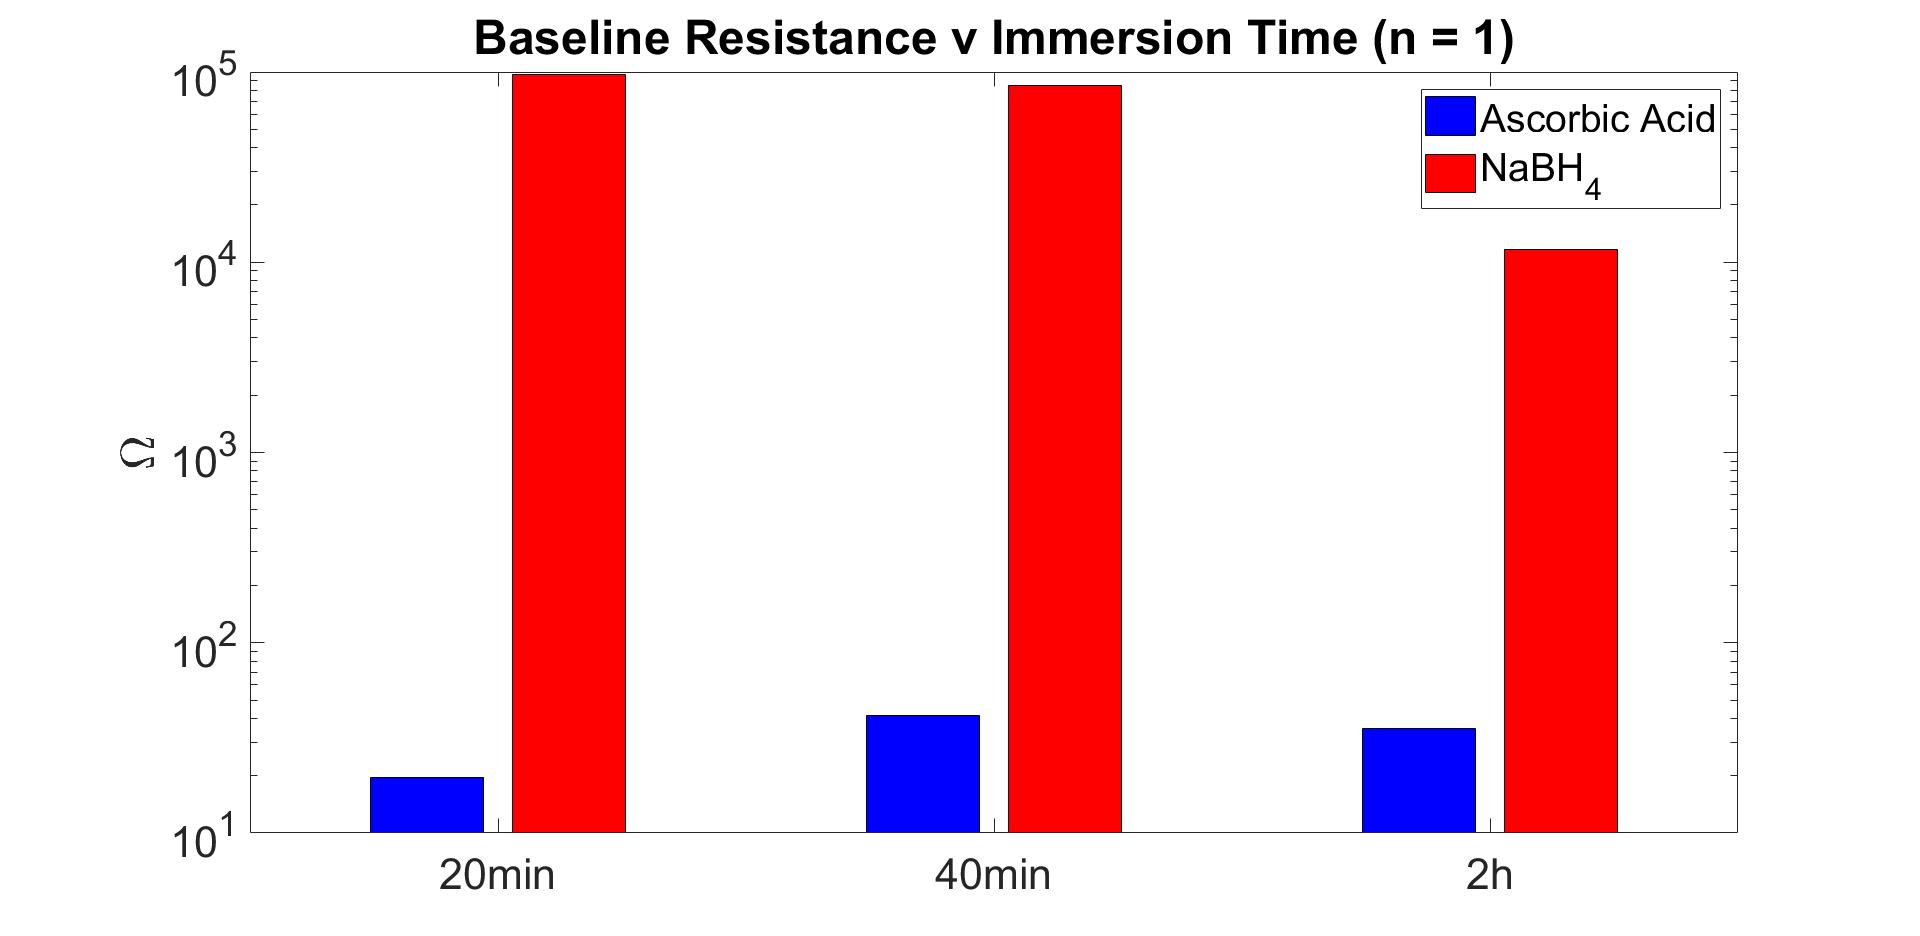
\includegraphics[width=1.2\textwidth]{./pic/tRedVR0.jpg}}
	\caption{Reducing Agent Immersion Times v Resistance}
	\label{fig:R0VtRed}
\end{figure}


\paragraph{NaBH4}
During Production we followed the standard procedure with the concentration stated. \ce{NaBH4} is known to hydrolyse in solute and therefore, the projected reactivity is reduced. To decrease premature hydrolation, the \ce{NaBH4}-solution was prepared just before usage and put on ice between production and use.\\

\begin{figure}[H]
	\centerline{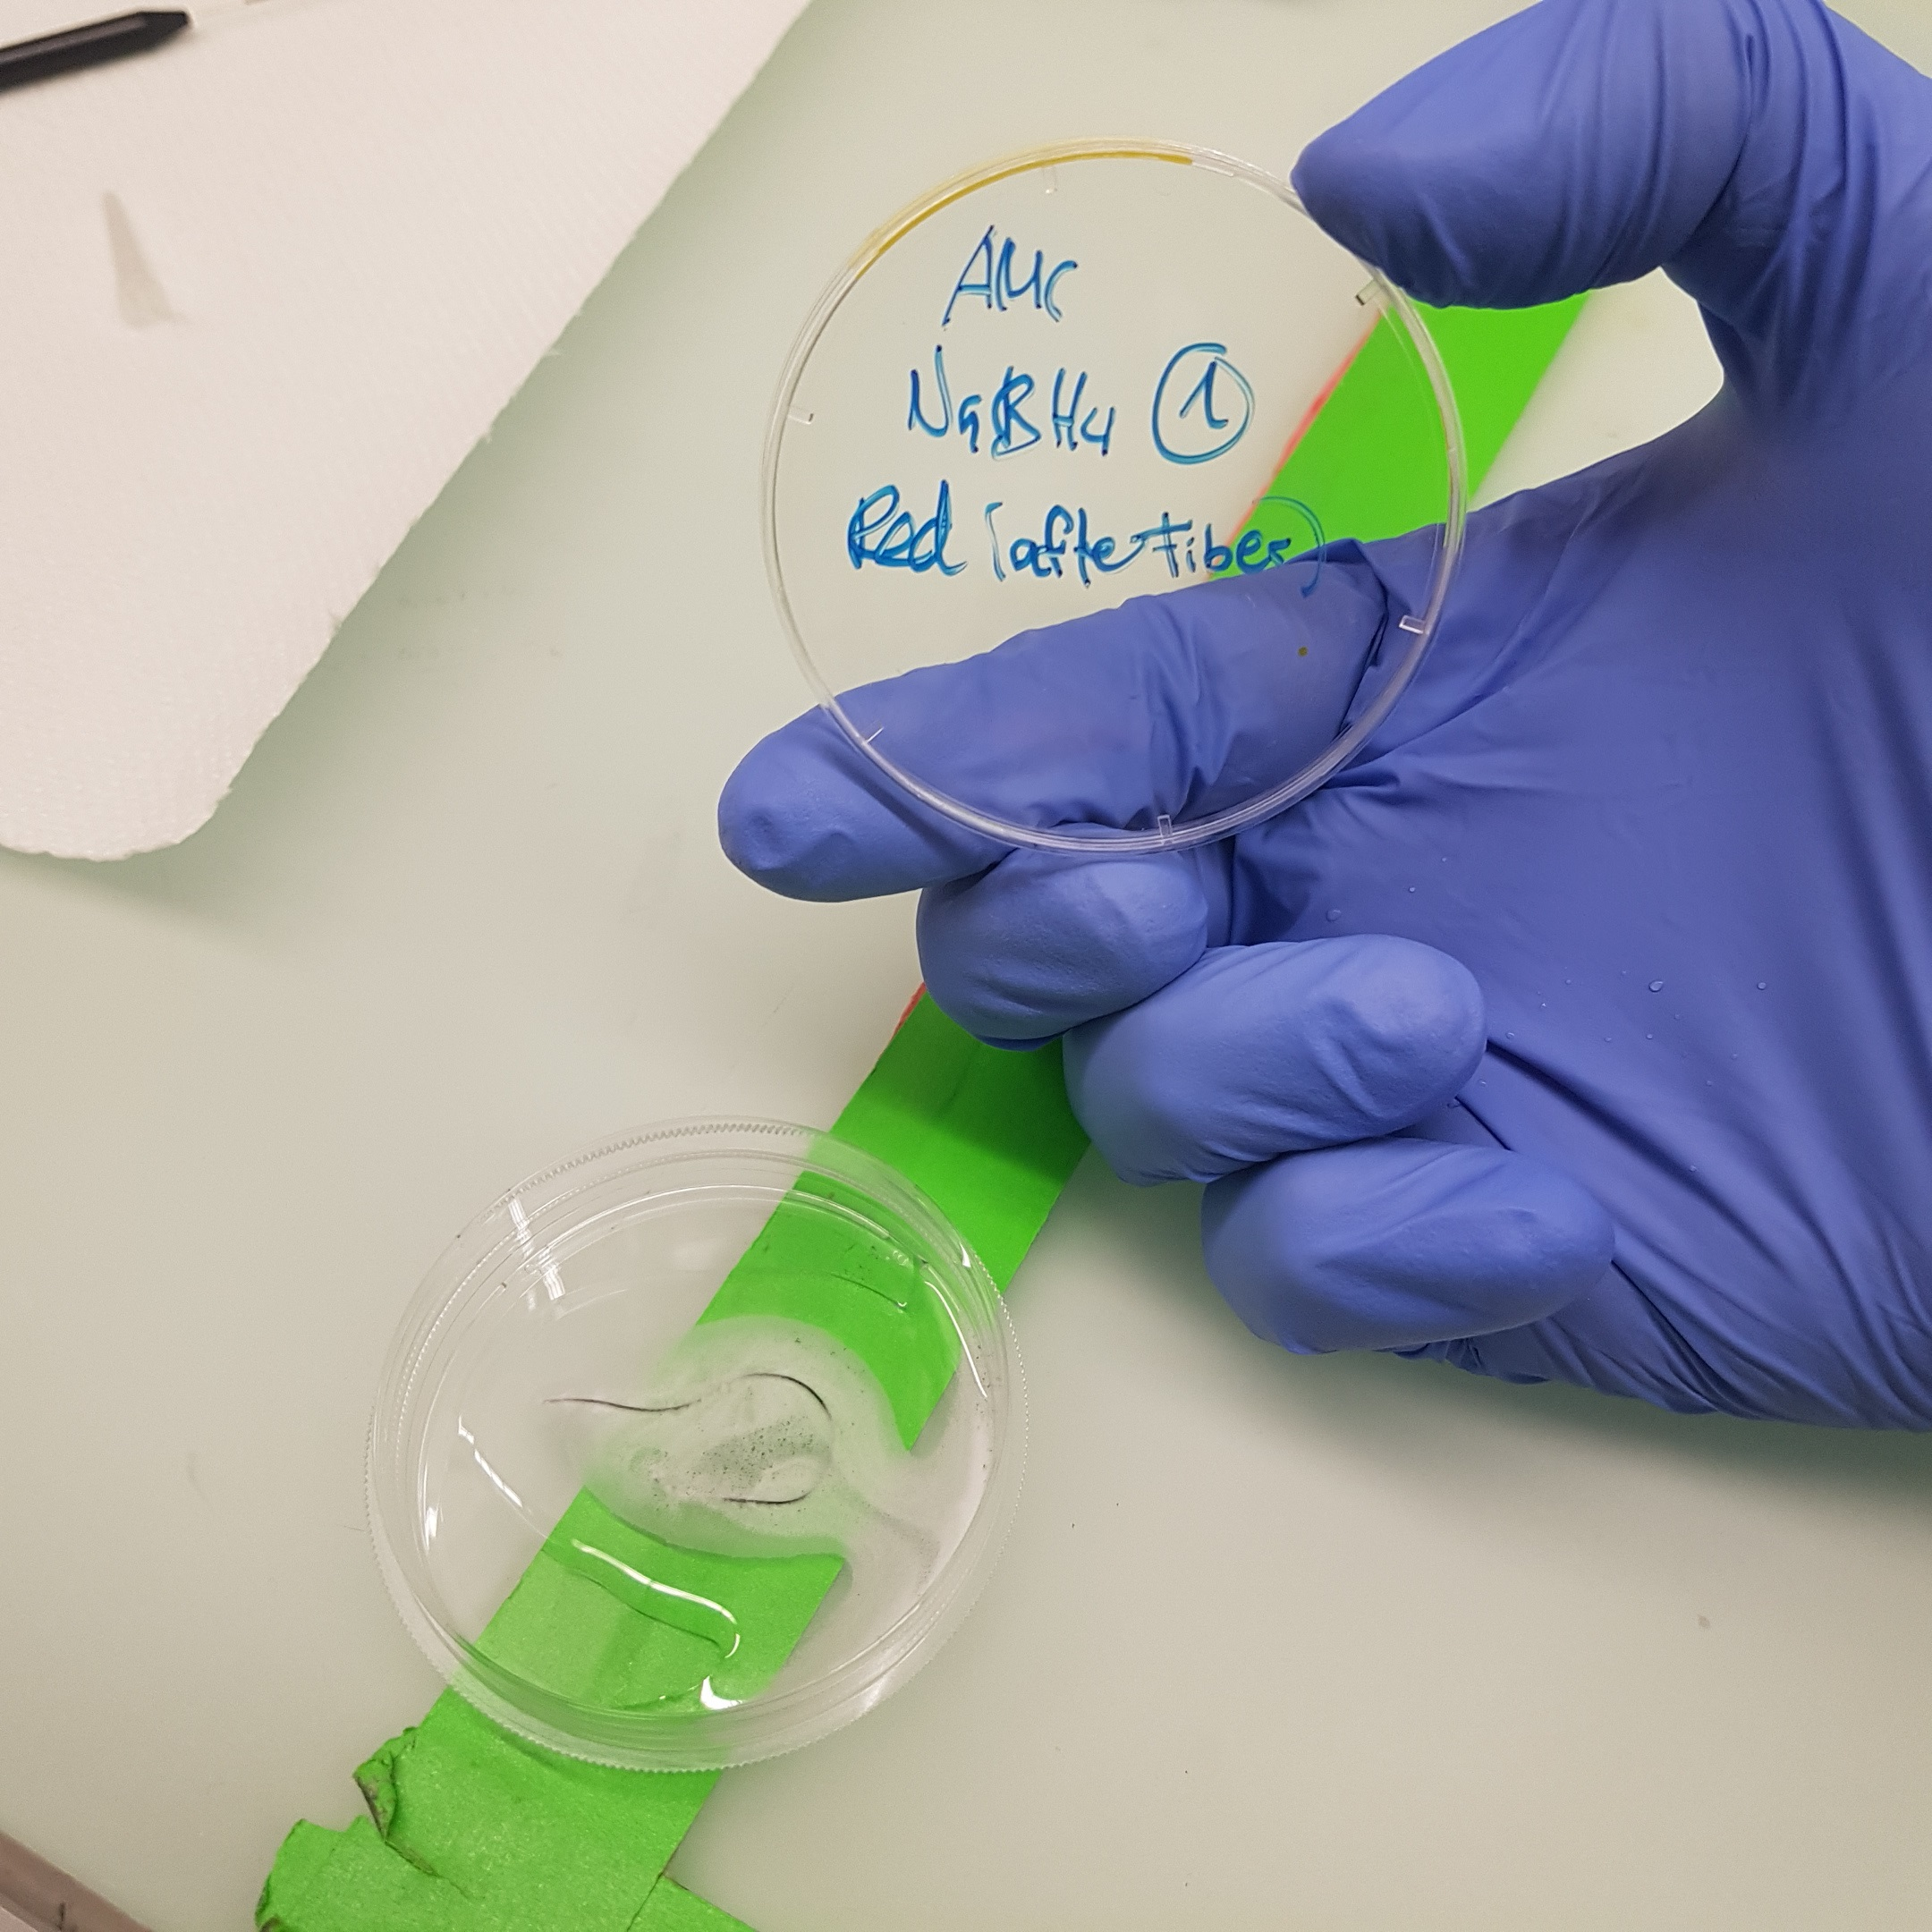
\includegraphics[width=0.7\textwidth]{./pic/BubblyPic.jpg}}
	\caption{Production of Hydrogen Gas upon Immersion}
	\label{fig:Bubbly}
\end{figure}

Upon immersion of fiber in \ce{NaBH4}, the production of bubbles could be observed as can be seen in figure \ref{fig:Bubbly}.

The following equation describes the oxidation-half reaction in this sample:

\begin{center}
\schemestart 
\ce{[BH4]-} + \ce{H+} + 3\ce{H2O}   \arrow{->} \ce{H3BO3} + 4\ce{H2{(g)}}, 
\schemestop\par 
\end{center}

With the stated concentration in table \ref{tab:RedAg}, we were able to measure conductivity in all three samples as can be seen in figure \ref{fig:R0VtRed}. We acknowledge the fact that one sample is not sufficient for any significant statement. Nevertheless, we see a tendency of a decreasing resistance when increasing the immersion time, exhibiting a time-dependency in this relation. As a general rule, chemical reactions are known to target a certain ratio between educt and product. \cite{ChemicalEqu} This principle could explain the time-dependency. The produced hydrogen gas evades the liquid reaction solution continuously as seen in picture \ref{fig:Bubbly}. This imbalance between reactant and product is counter-steered by a shift towards the product side present in the solution, which over time would lead to a steady-state, where the increased concentration of \ce{H3BO3} compensates for the lack of \ce{H2{(g)}}. However, as long the reaction did not reach the steady state, gold atoms will be produced and nuclei will grow. This implies the decrease in resistance whose end is marked by a critical point that is governed either by reaching the ratio described above or the nanoparticle size, which grows to over the optimal size.

Scanning Electron Microscopy (SEM) pictures showed a largely heterogeneous distribution of nanoparticles. However, EDS analysis of the crosssection of the fiber shown in appendix on page \pageref{SEMAppendix} reveals gold coating. 

\paragraph{\text{\ce{NaBH4}/\ce{NaOH}}}
Production was done according to protocol and with the concentration stated in table \ref{tab:RedAg} on page \pageref{tab:RedAg}. As already mentioned in the \ce{NaBH4}-group, we wanted to decrease premature hydrolation. This was done by both - separate preparation of both chemicals before mixing when immersing the sample and also by cooling it before usage. We were not able to measure any conductivity in this sample. This is inconclusive, considering, that \ce{NaBH4} and \ce{NaOH} are similar substances.


\paragraph{Hydroxylamine}
Production was done according to protocol and with the concentration stated in table \ref{tab:RedAg} on page \pageref{tab:RedAg}. No conductivity was measured. Nevertheless, SEM pictures revealed successful reduction of gold into round nanoparticles that at some location formed large colloids (see \ref{fig:SEMPicCombo}.4). Following the principle of Occam's razor, we hypothesise that in the process of the reaction, eventually, the nanoparticles grew to big and subsequently "fell off" the fiber. This explains the phenomenon of no measurable conductivity even with apparent presence of particles. \hfill \newpage


\paragraph{Ascorbic Acid}

\begin{wrapfigure}{r}{0.4\textwidth}
	\begin{center}
		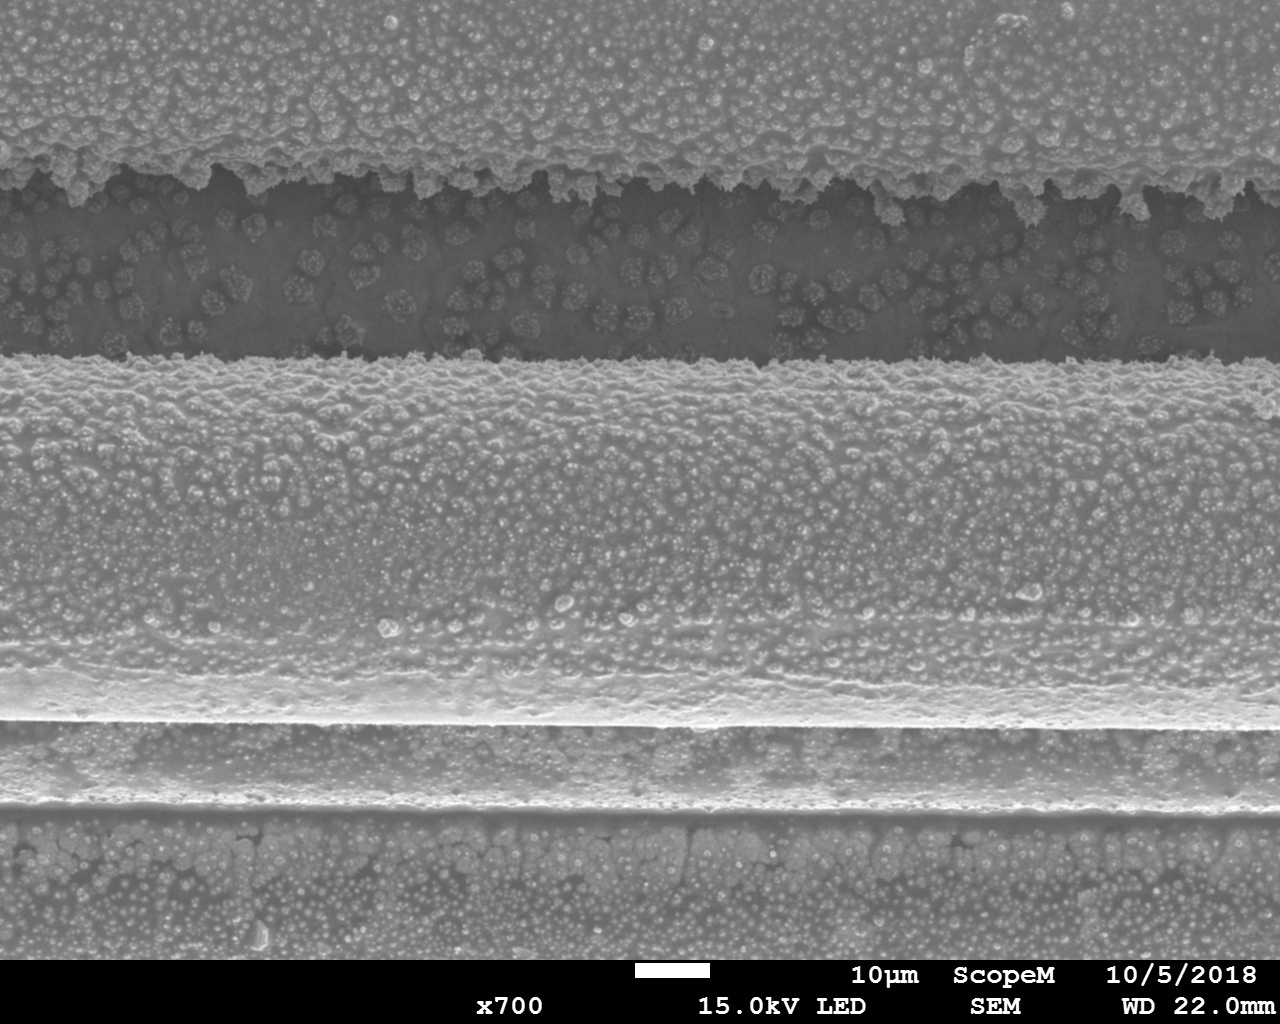
\includegraphics[width=0.38\textwidth]{./pic/AscAcid_1_3_10mum.png}
	\end{center}
	\caption{\label{AscAcidFibre} SEM Pictures of Ascorbic Acid Fiber}	
\end{wrapfigure}


Production was done according to protocol and with the concentration stated. The conductivity measured was 33 $\Omega$ on average ($\approx$ $10\frac{\Omega}{cm}$) and outperforms the next best reducing agent by three orders of magnitude in the described setup. This result is particularly interesting when considering the structural similarity between Ascorbic Acid and Glucose, which did not perform. However, the SEM Pictures reveal a clear distinction of the surface of the fiber. Additional EDX-analysis on page \pageref{SEMAppendix} corroborates the findings, albeit there is no gold deposition found inside of the fiber. One possible explanation is that the PUR is soaked with gold solution, but the AscAc is possibly sterically hindered from entering. 


\paragraph{Citric Acid}

\begin{wrapfigure}{l}{0.4\textwidth}
	\begin{center}
		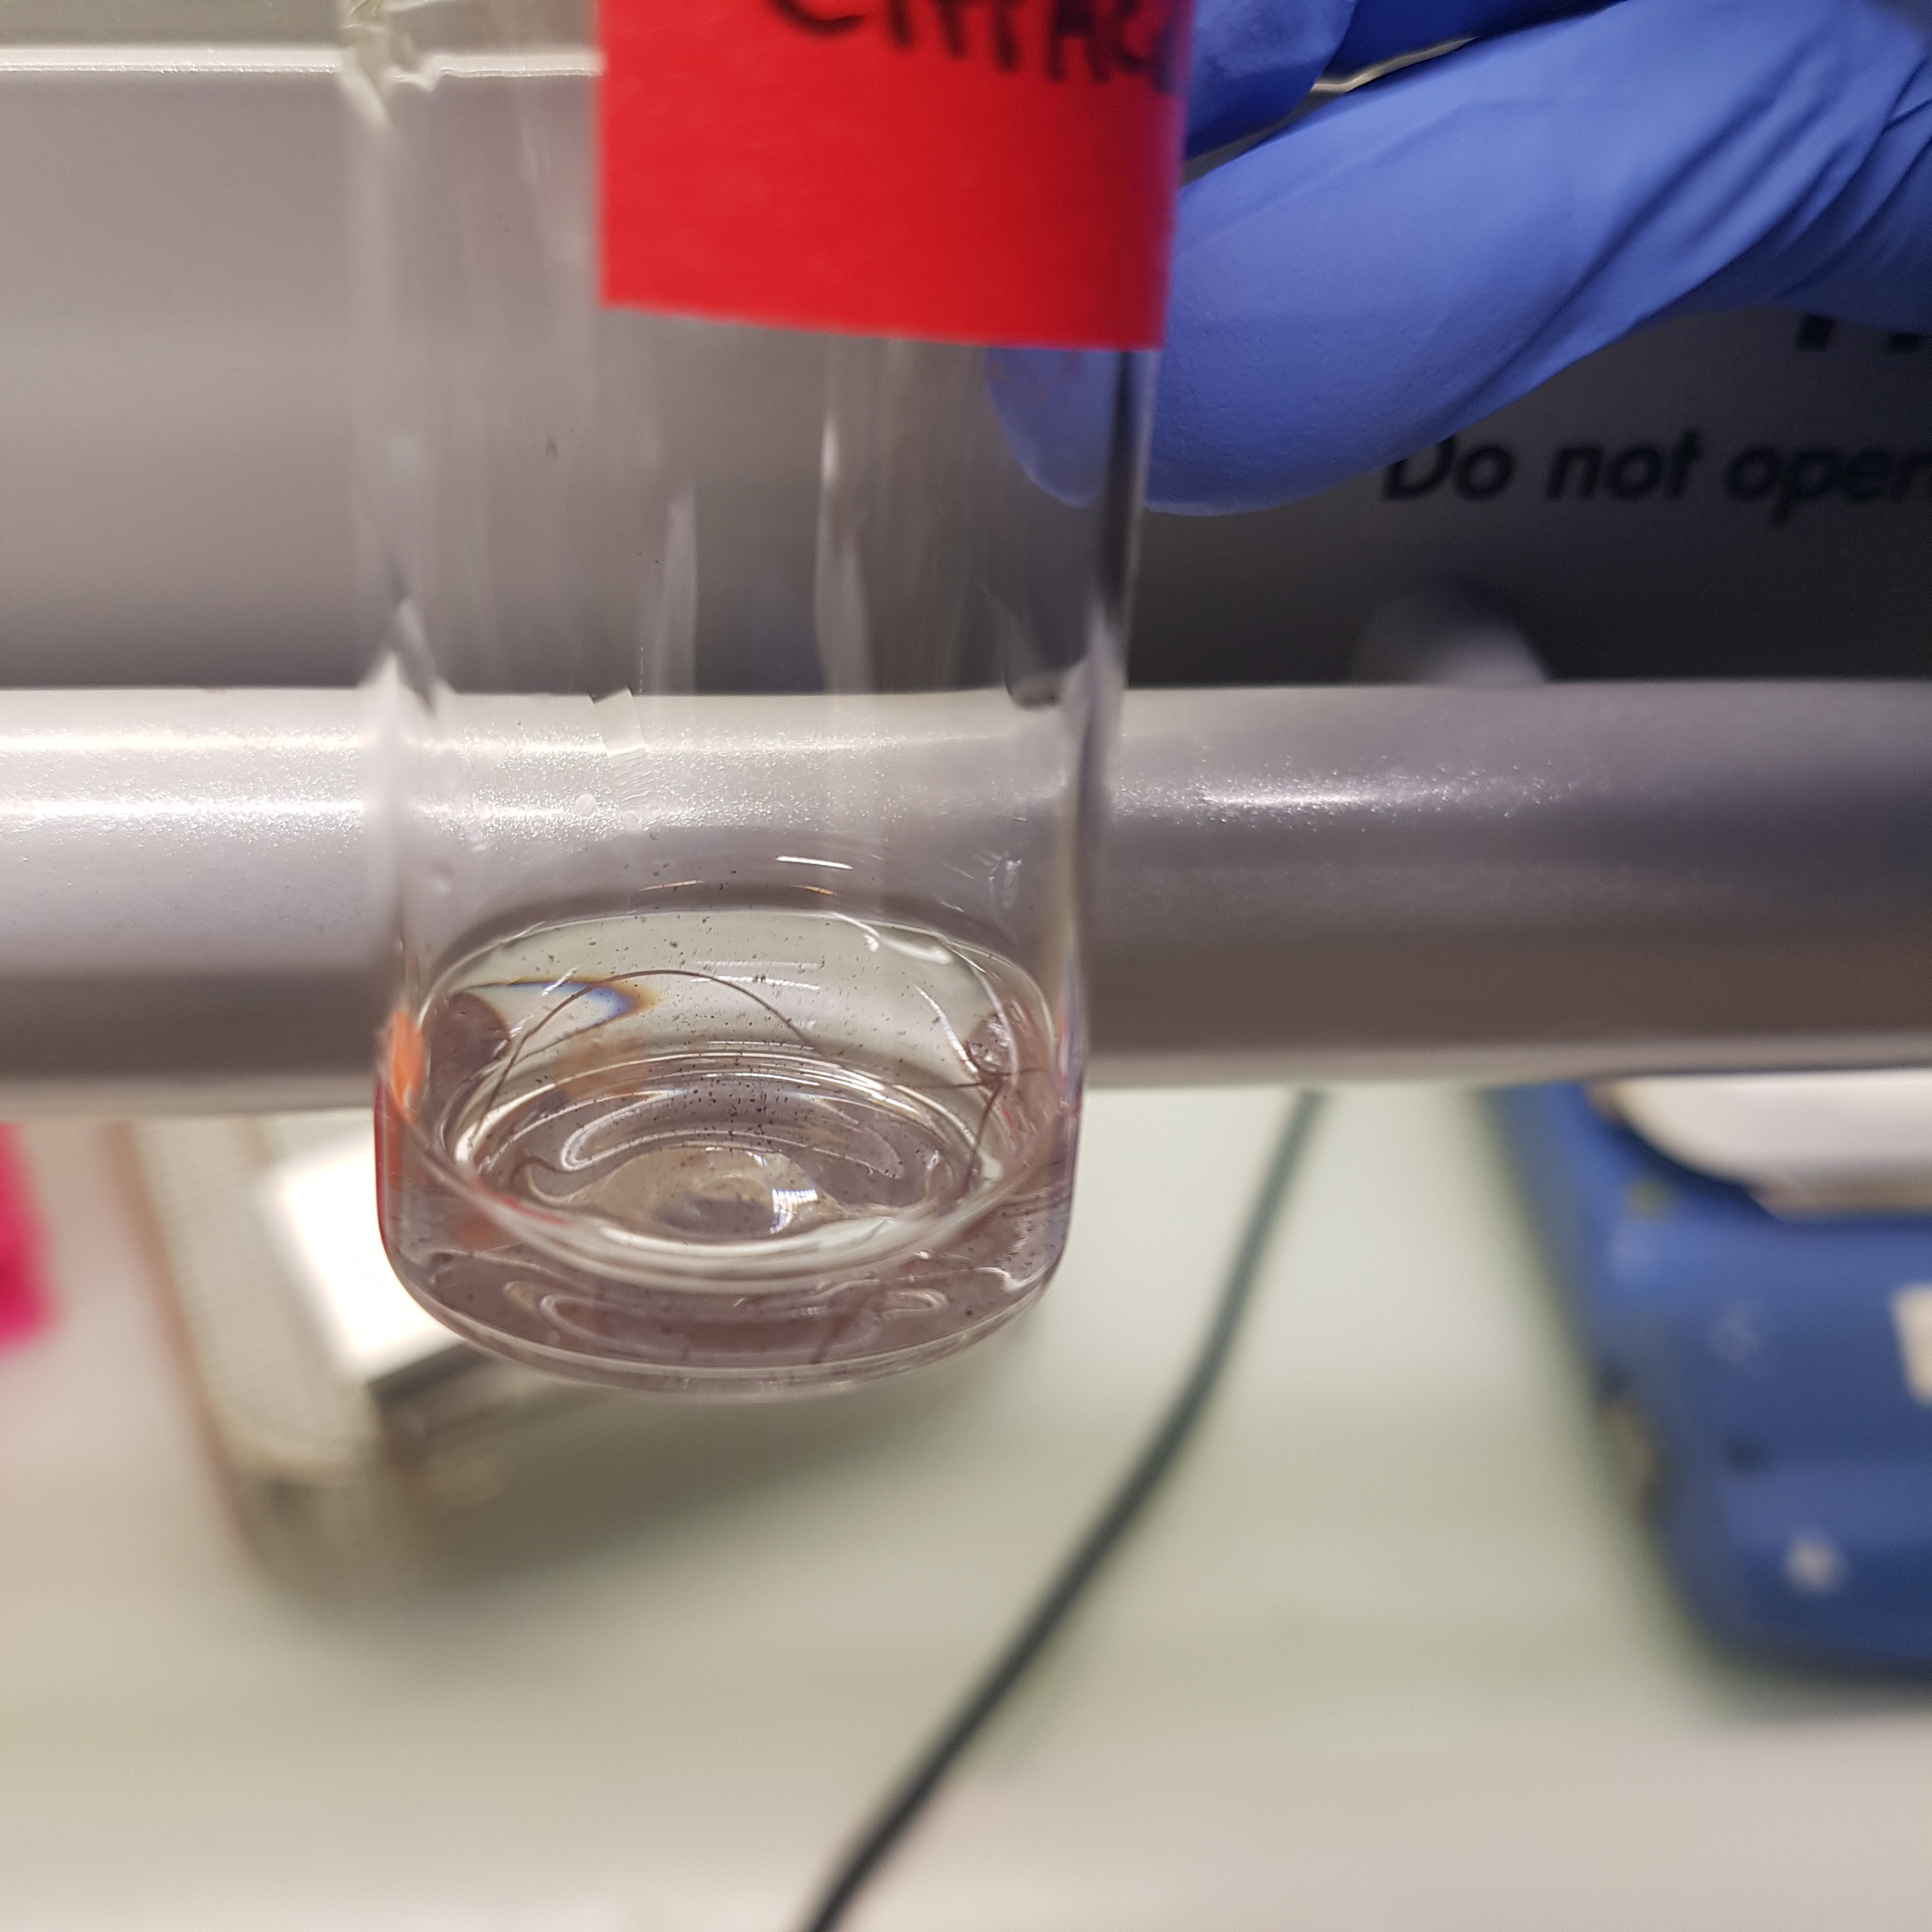
\includegraphics[width=0.38\textwidth]{./pic/CitricAcidViol.jpg}
	\end{center}
	\caption{\label{CitrcAcFibre} Citric Acid Reaction Liquid}	
\end{wrapfigure}


The citric acid protocol was slightly changed, upon suggestion by work done by Kimling \cite{Kimling} to include an initiating element to facilitate the formation of nuclei, which then - according to explanation found in chapter \ref{subsec:Perc} - should suffice for produced gold atoms to associate to the nucleus and finally nanoparticles to grow. The identified initiators where heat-exposition and UV-irradiation. For each of those two subgroups, only one sample was prepared.

We prepared the heat exposition group following standard procedure up until the immersion of the fiber in the reducing agent (i.e. citric acid in this case). Using the hot plate, we prepared the citric acid solution to be between 100-120 \degree C, before the fiber was immersed. Over the course of 35 minutes the solution changed from faintly blue and turbid to a clear solution with red particles floating in the solution. A picture of the solution after letting it cool down is shown on page \ref{CitrcAcFibre}. The described behaviour replicates the description by Frens\cite{Frens}. Yet, we were not able to measure current.

Using a Demetron Optilux 500, we irradiated one sample after immersion  citric acid solution for 2 minutes. The picture \ref{fig:BubblyAndSad}.1 on page \pageref{fig:BubblyAndSad} shows the emergence of bubbles at the fiber-solution-interface during irradiation. Comparison with a control citric acid group, where bubble formation was absent, leads to conclusion the phenomenon is caused by the irradiation. However, the integrity of the fiber was impaired. Attempts to take it out the petri dish, showed that the polyurethan fiber was thinned out substantially and sticked on the petri dish (see fig. \ref{fig:BubblyAndSad}.2).  Obviously, there was an influence of the UV-light on the fiber. Further experiments with variable irradiation times and/or intensities, could lead to a more thorough explanation. No conductivity measurement was done in this group.

 \begin{figure}[H]
	\centerline{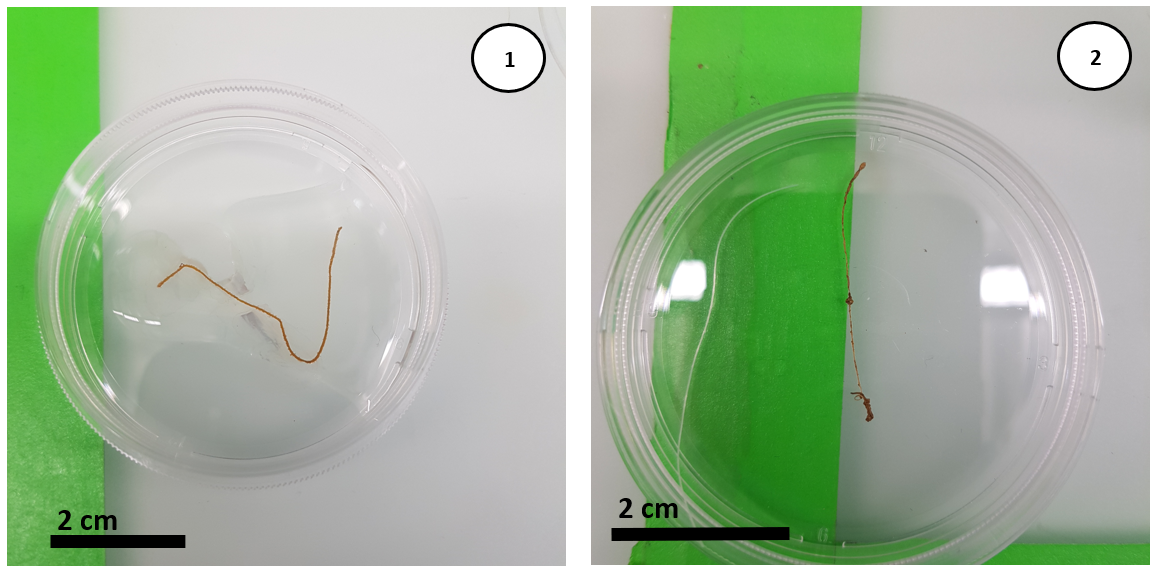
\includegraphics[width=\textwidth]{./pic/BubbleAndSad.PNG}}
	\caption{\\
		1) Bubble Formation After UV Irradiation 2) Loss in integrity}
	\label{fig:BubblyAndSad}
\end{figure}
\vfill \newpage


\paragraph{Glucose}

\begin{wrapfigure}{r}{0.4\textwidth}
	\begin{center}
		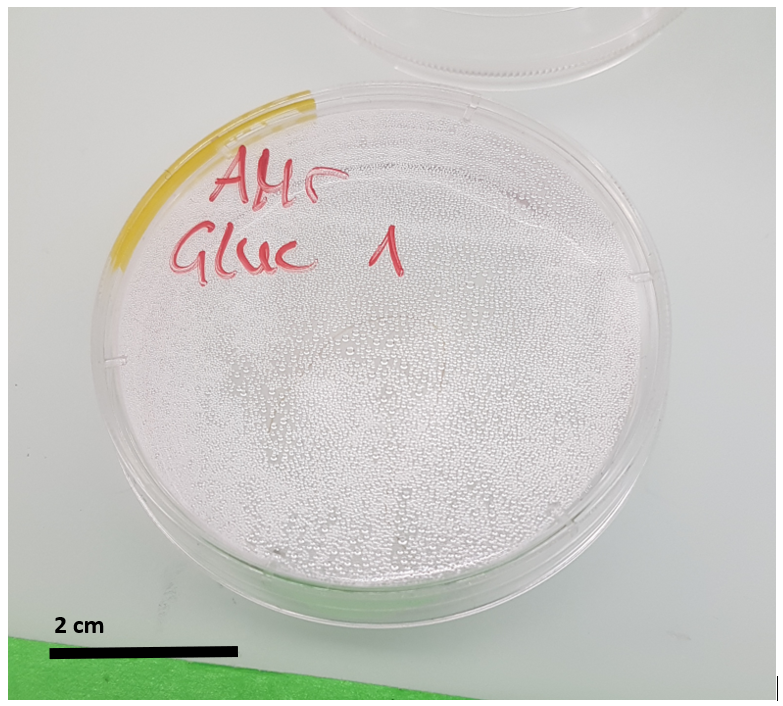
\includegraphics[width=0.38\textwidth]{./pic/Gluc.PNG}
	\end{center}
	\caption{\label{Gluc} Condensed Reducing Agent in Glucose Sample}	
\end{wrapfigure}
Upon suggestion by Kimling \cite{Kimling}, we kept the reducing agent solution at around 30 \degree C during the whole immersion time, using the hot plate. After 15 minutes, some of the solution clearly 
 visible condensed on the closing lid of the petri dish. We were not able to measure any conductivity in this sample.
However, SEM pictures revealed the formation of gold nanoparticles as can be seen in figure \ref{fig:SEMPicCombo}.4. The nanoparticles seem to have crack like indentations. However, we are not able to asses the quality any further. Further experiments with variable temperature, heating times and glucose concentration may provide more information on the origin of this behaviour.\\
All reducing agents tested effectuated a change in fiber colour when following the described protocol. If not stated otherwise the sample did not lead to any behaviour that was worth noting, neither when analysing the reducing agent solution after sample immersion nor the fiber by eye.

However, due to the fact that no reducing agent but \ce{NaBH4} and \ce{AscAc} did lead to conduction in our fibers, we also conclude that the sheer reduction of gold is not enough to functionalise our fiber with conductivity. In order to get closer to a satisfying explanation for the relationship between the reducing agents and the conductivity of the fiber, we have to further characterize the gold nanoparticles by size, shape and spatial distribution and then try to derive the rules governing the dynamic. Further experiments could elucidate which of these factors weigh how much into the equation that explains conductivity in our fibers. 



 \begin{figure}[H]
 	\centerline{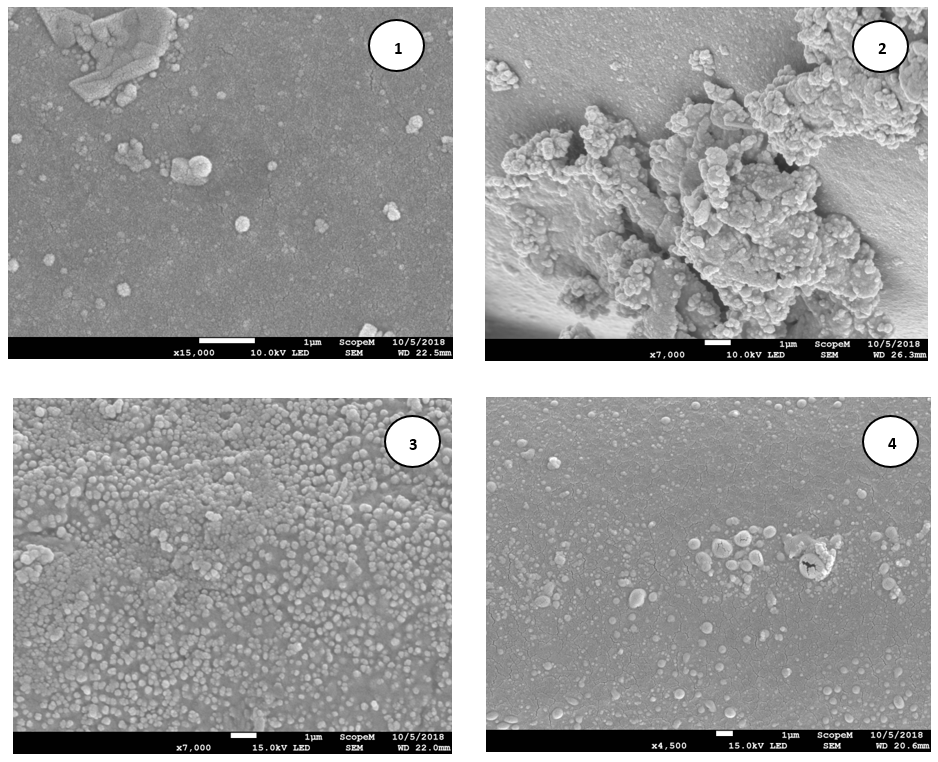
\includegraphics[width=\textwidth]{./pic/SEM/Combination.png}}
 	\caption{SEM Pictures\\
 	1) \ce{NaBH4} 2) Hydroxylamine 3) Ascorbic Acid 4) Glucose}
 	\label{fig:SEMPicCombo}
 \end{figure}
 

%\hfill \newline

All reducing agents tested effectuated a change in fiber colour when following the described protocol. If not stated otherwise the sample did not lead to any behaviour that was worth noting, neither when analysing the reducing agent solution after sample immersion nor the fiber by eye.

However, due to the fact that no reducing agent but \ce{NaBH4} and \ce{AscAc} did lead to conduction in our fibers, we also conclude that the sheer reduction of gold is not enough to functionalise our fiber with conductivity. In order to get closer to a satisfying explanation for the relationship between the reducing agents and the conductivity of the fiber, we have to further characterize the gold nanoparticles by size, shape and spatial distribution and then try to derive the rules governing the dynamic. Further experiments could elucidate which of these factors weigh how much into the equation that explains conductivity in our fibers. 

As can be seen in the SEM pictures in figure \ref{fig:SEMPicCombo}, we can partially explain the conductivity by uniformity in spatial distribution and size of the nanoparticles. However, the apparent similarity between \ref{fig:SEMPicCombo}.1 and \ref{fig:SEMPicCombo}.4 shows that this is not sufficient of an explanation, since they did not peroform equally. In the case of \ref{fig:SEMPicCombo}.2, we see a large complex, that seems to be stem from many congregated metallic particles, following the explanation given in chapter \ref{subsec:Perc}. 

\subsection{Optimisation}

Encouraged by the good results we decided to optimise for AscAc before making baseline resistance tests for new reducing agents. Additionally, we now took not only the baseline resistance into account but also its behaviour when put under strain forces. This measurement reflects now more the true use case and should reduce misdirected optimisation. The five independent variables defined in chapter are now reduced to four. If not different stated, following applies: 

\begin{center}$c_{AscAc}=0.19M$, $t_{AscAc}=20min$, $c_{Gold}=0.25M$ and $t_{Gold}=1h$
\end{center}
Next we assigned each of those independent variables an anticipated effect size. By intuition we assigned them in the following order, where $>$ marks "has the bigger anticipated effect size than":

\begin{equation}
    c_{AscAc} > c_{Gold} > t_{AscAc} > t_{Gold}
\end{equation}

\subsubsection{Variation of Gold Concentration}

In this experiment we investigated on the strain-resistance behaviour in three different groups, where the only thing that was changed between groups was $c_{Gold}$ to be either $0.025M$, $0.25M$ or $0.6M$.

\begin{figure}[H]
    \centerline{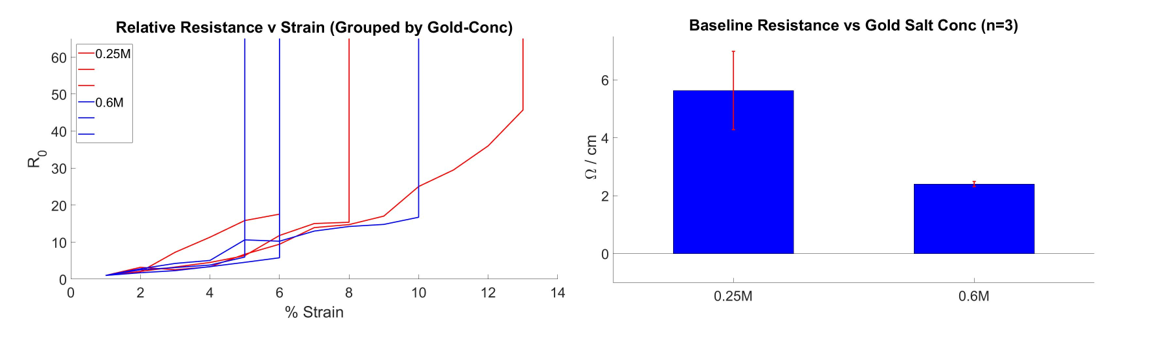
\includegraphics[width=\textwidth]{./pic/R0vGoldConc.PNG}}
    \caption{Variation of Gold Concentration}
    \label{fig:GoldConc}
\end{figure}



The $0.025M$-samples did not lead to measurable conduction. The result of the baseline resistance seemingly favours a higher gold concentration. However, the data of strain resistance does not allow for a similarly clear statement, neither when plotting the absolute resistance nor when plotting the normalised one, as we see in figure \ref{fig:GoldConc}, right. The sudden peak out of the plotted range mark the critical point, where conductivity in the fiber was lost and no current was measured. Relaxation of strain also led to regain of measurable conductivity similar to a priori values (not shown). Intuitive reasoning where a higher gold concentration leads to lower baseline resistance but faster loss of conductivity due to more rigid behaviour, doesn't seem to manifest itself in the acquired data.

\subsubsection{Variation of Reducing Agent}


\begin{figure}[H]
    \centerline{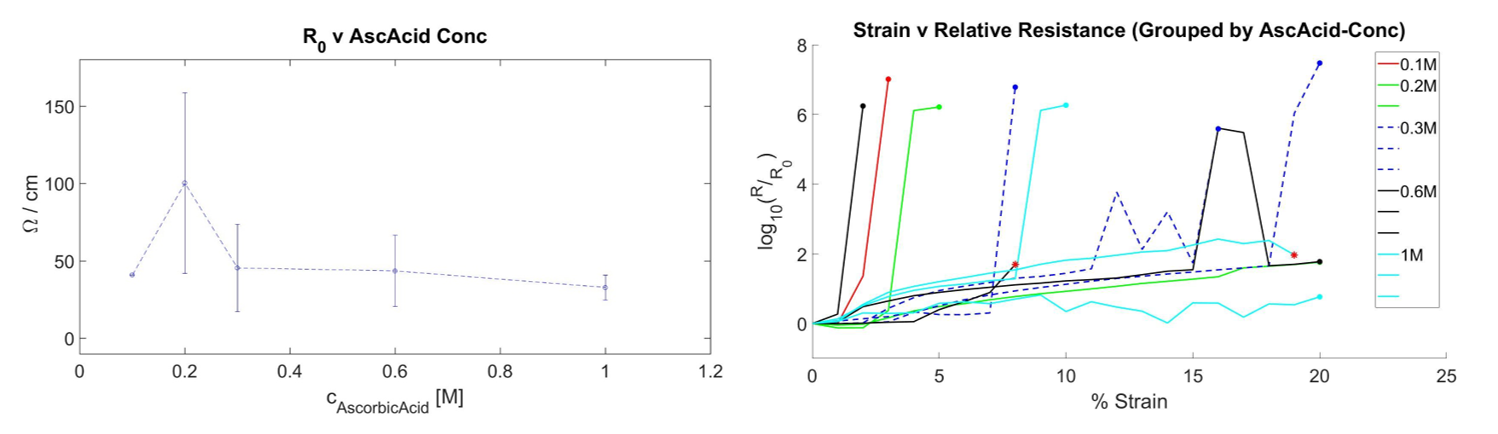
\includegraphics[width=\textwidth]{./pic/StrainVAscAcidConc_2.PNG}}
    \caption{Variation of Gold Concentration}
    \label{fig:StrainVAscAcidConc}
\end{figure}


In the next experiment we set up 15 samples and divided them in 5 groups, which had all the same experiment paramters, but the $c_{AscAc}$.
We varied the AscAc-concentration to be either $0.1M, 0.2M, 0.3M, 0.6M$  or $1M$, respectively. In this experiment, we used the optimized protocol described on page 10. Sadly, this lead to only inconclusive data as seen in the figure above. Similar to the plot \ref{fig:GoldConc}, the sudden surge in resistance marks the critical point where conductivity was lost. Additionally, at the red crosses, we had to manually stop the measurement due to the resistance measured jumping between multiple orders of magnitude, which wasn't representative. The jumping most probably was caused by a intermittent contact, which might could be ameliorated by a elastomeric layer that would enclose the fiber. 